\section{History}
The development of both the electric motor and generator follow similar timelines, since their reciprocity was discovered soon after the invention of the first motor.

    \subsection{Electric Motor}

    \begin{figure}[!ht]
        \begin{center}
            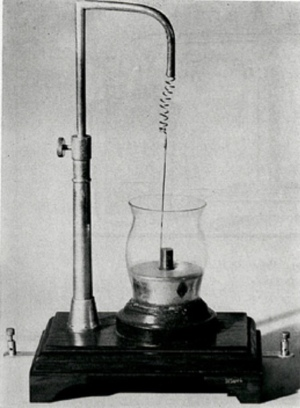
\includegraphics[width=0.35\textwidth]{figures/history/rotating_wire.jpg}
            \label{fig:faraday}
        \end{center} \caption{Rotating Wire by Faraday, 1821}
    \end{figure}

    \noindent
    Michael Faraday is known for contributing to the earliest development models of the generator. His 1821 prototype consisted of a stiff wire hanging down into a glass vessel half filled with mercury over a bar magnet. When connected to a battery, the wire would rotate clockwise due to its induced field interacting with the magnetic field. \cite{firstmotor} The development of his prototype sprung from earlier observations by Hans Christian Oersted on the deflection of a compass needle by electric currents in 1820, and the invention of the solenoid by Andre-Marie Ampere in the same year. \cite{solenoid_ref} The magnetic field generated by the electric current were made stronger with the invention of the electromagnet by William Sturgeon in 1826 by inserting an iron core in the solenoid. \cite{em_ref} \\

    \begin{figure}[!ht]
        \begin{center}
            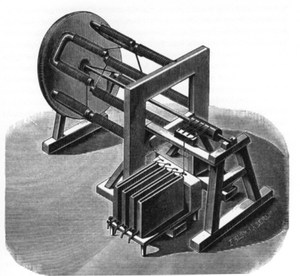
\includegraphics[width=0.35\textwidth]{figures/history/jacobi.jpg}
            \label{fig:jacobi}
        \end{center} \caption{The First Real Electric Motor by Jacobi, 1834}
    \end{figure}

    \noindent
    Several models were developed and improved upon since the primitive models, until in 1834 when the electric motor was deemed commercially successful by being able to perform useful tasks. Moritz Hermann Jacobi constructed his motor to lift a weight of of 10 - 12 pounds with a speed of 1 foot per second, which is equivalent to about 15 watts of mechanical power. \cite{jacobi} Jacobi’s model is considered the first real and usable electric motor.

    \subsection{Electric Generator}

    \begin{figure}[!ht]
        \begin{center}
            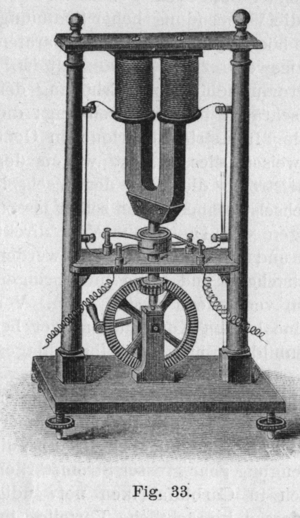
\includegraphics[width=0.2\textwidth]{figures/history/pixii.jpg}
            \label{fig:pixii} \caption{Pixii's First Generator, 1832/1833}
        \end{center}
    \end{figure}

    \noindent
    Concurrently, the development of electric generators was already under way. Michael Faraday was also responsible for discovering electromagnetic induction in 1831, the inverse of the earlier observation by Oersted. Oersted discovered the generation of magnetic fields from moving currents, while Faraday observed the reciprocal of the process and began documenting the phenomenon. The concept was demonstrated a year later by Hippolyte Pixii, when he noticed how running an electric motor backwards would induce current. He builds the first apparatus for generating pulses of direct current out of a rotation. \cite{pixii} Commutators and brushes were added in William Ritchie’s generator around the same time. Several improvements were attempted after the primitive designs, but mankind had to wait almost 25 years for an electric generator powerful enough for commercial use.\\

    \begin{figure}[!ht]
        \begin{center}
            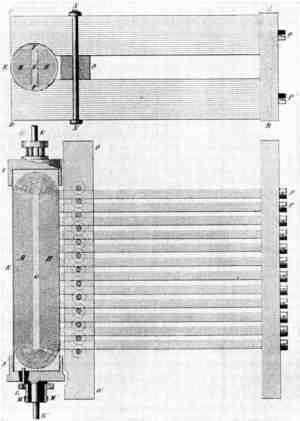
\includegraphics[width=0.2\textwidth]{figures/history/siemens.jpg}
            \label{fig:siemens} \caption{Double-T Armature Winding by Siemens, 1857}
        \end{center}
    \end{figure}

    \noindent
    In 1856, Werner Siemens builds an electric generator with a double-T armature winding. He became the first inventor to place the windings in slots, a design that almost all electric motors to date are built with. \cite{siemens} Around a year later, he develops the dynamo-electric machine based on his double-T armature capable of generating sufficient power. The current generated was however in pulsating direct current. Friedrich von Hefner-Alteneck improves Siemens’ design by wrapping wire around a cylinder-shaped anchor to produce a smooth DC current. \cite{hefner} 

    \subsection{Contributions to Society}
    The introduction of the electric motor and electric generator laid down the foundations for most of the technological advancements in society to date. The electricity that is provided in our homes, workplaces, commercial and public areas is generated through electric generators in power plants. Almost all home appliances, such as refrigerators, air conditioners, fans, vacuum cleaners, blenders, and computer hard drives operate with at least one electric motor inside them. Society today would not be able to function properly without the benefits of motors and generators.

\clearpage
